\documentclass[tikz,border=6pt]{standalone}
\usepackage[T1]{fontenc}
\usepackage[utf8]{inputenc}
\usepackage{import}
\subimport{layers/}{init.tex}
\usetikzlibrary{arrows.meta,positioning}
\definecolor{ink}{HTML}{242629}
\definecolor{muted}{HTML}{59616a}
\definecolor{panel}{HTML}{f6f6f3}
\definecolor{blue}{HTML}{dfeaf5}
\definecolor{peach}{HTML}{f7cdae}
\definecolor{green}{HTML}{a9ce91}
\definecolor{yellow}{HTML}{ffe49b}
\definecolor{purple}{HTML}{d5c5e8}
\definecolor{white}{HTML}{ffffff}
\definecolor{heat}{HTML}{e89a50}
\definecolor{offset}{HTML}{a6bdd8}
\definecolor{size}{HTML}{ddc66e}
\definecolor{yaw}{HTML}{a8c983}
\definecolor{iou}{HTML}{b6a1cd}
\begin{document}
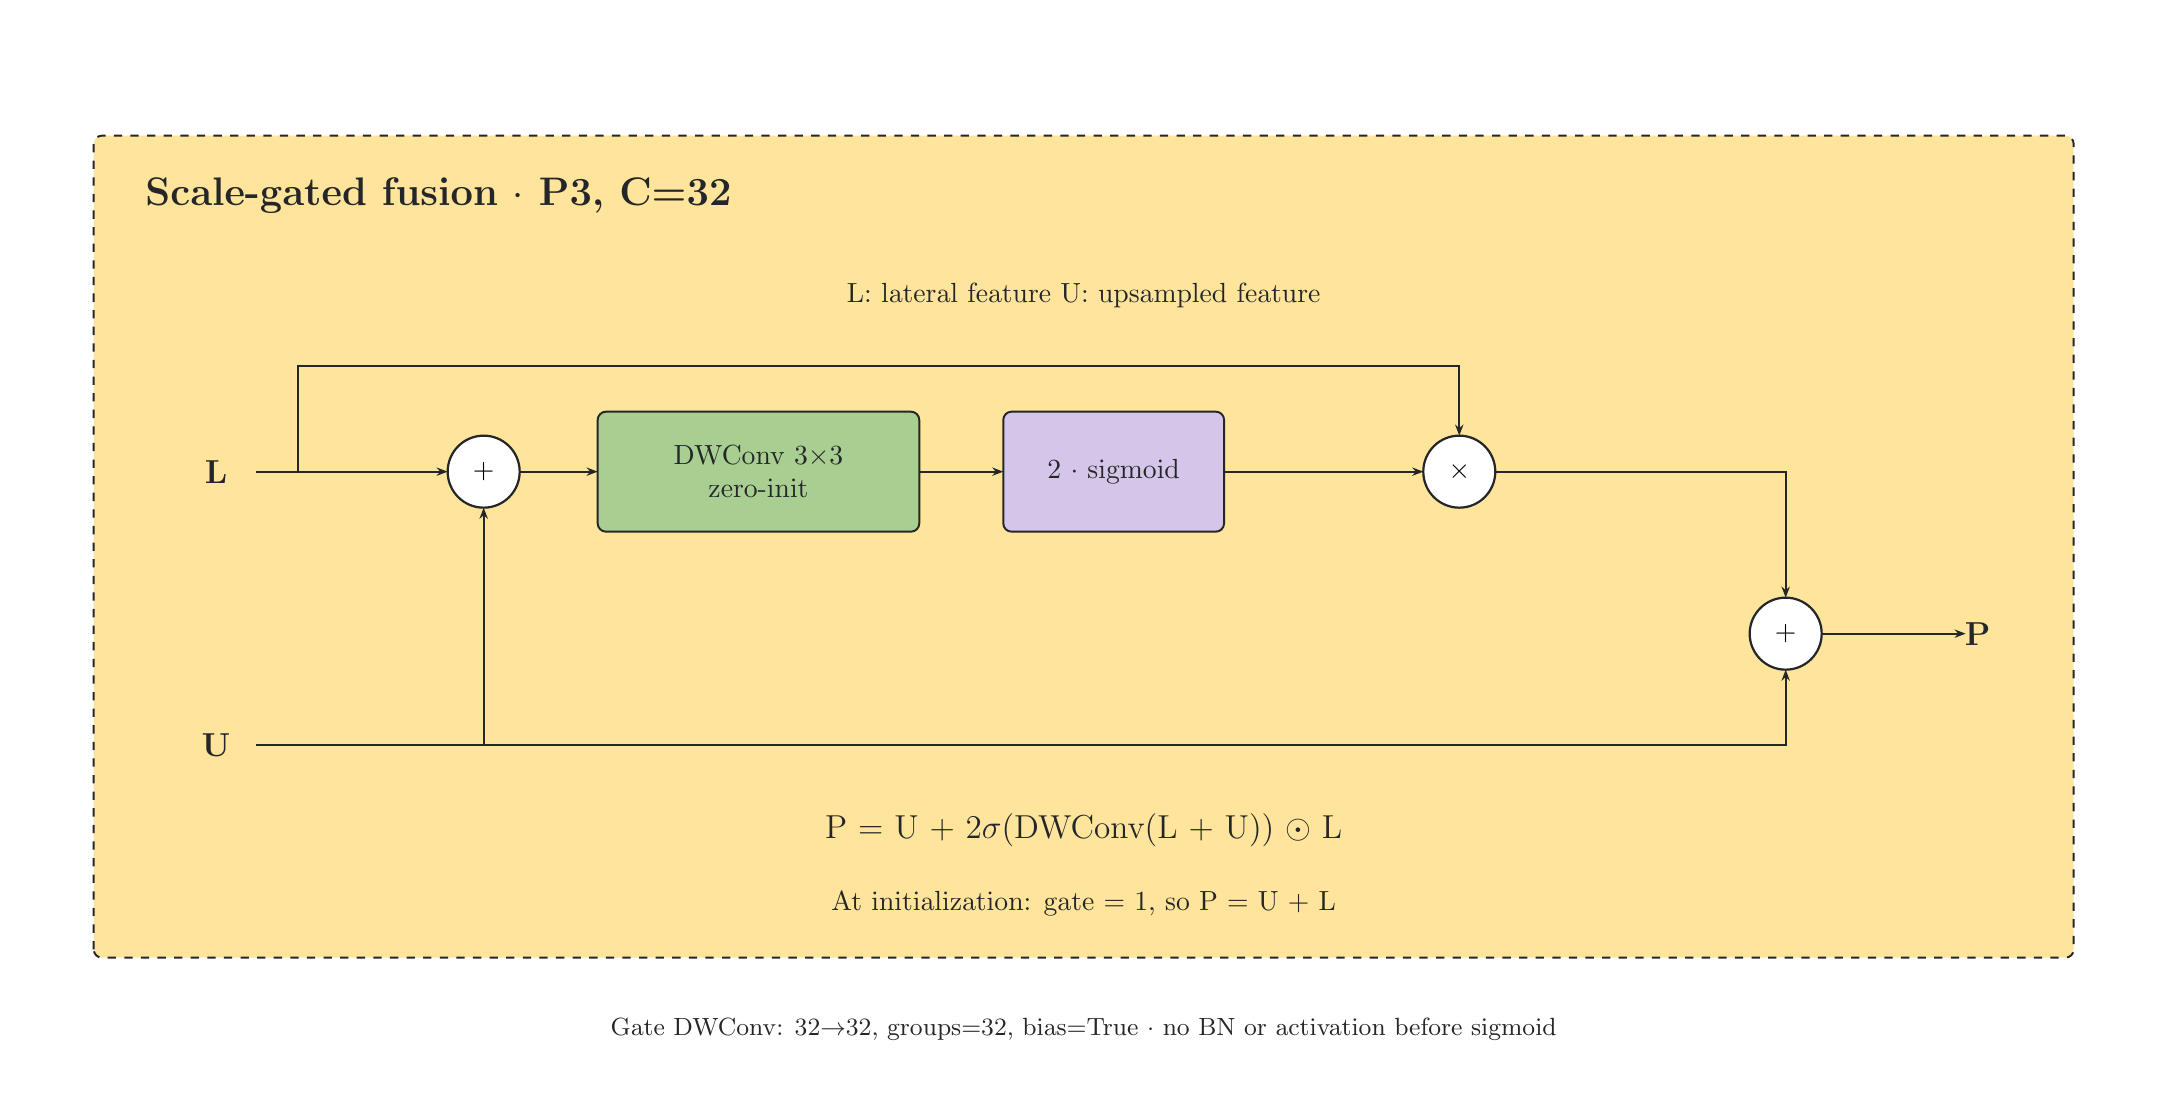
\begin{tikzpicture}[x=1.524cm,y=1.524cm,z={(0.9906cm,0.73152cm)}]
\path[use as bounding box] (0,0) rectangle (17.6,8.7);
\draw[draw=ink,fill=yellow,rounded corners=3pt,line width=.7pt,dashed] (0.5500000000000007,0.9500000000000002) rectangle (17.05,7.8);
\node[anchor=west,align=left,text=ink,font=\fontsize{14}{16.8}\selectfont \bfseries ] at (0.9000000000000021,7.3) {Scale-gated fusion $\cdot$ P3, C=32};
\node[anchor=center,align=center,text=ink,font=\fontsize{10}{12.0}\selectfont ] at (8.8,6.470000000000001) {L: lateral feature    U: upsampled feature};
\node[anchor=center,align=center,text=ink,font=\fontsize{13}{15.6}\selectfont \bfseries ] at (1.5700000000000003,5.0) {L};
\node[anchor=center,align=center,text=ink,font=\fontsize{13}{15.6}\selectfont \bfseries ] at (1.5700000000000003,2.7199999999999998) {U};
\draw[fill=white,draw=ink,line width=.8pt] (3.8000000000000007,5.0) circle (0.3);
\node at (3.8000000000000007,5.0) {+};
\draw[-{Stealth[length=4pt]},draw=ink,line width=.7pt] (1.9000000000000021,5.0) -- (3.5,5.0);
\draw[-{Stealth[length=4pt]},draw=ink,line width=.7pt] (1.9000000000000021,2.7199999999999998) -- (3.8000000000000007,2.7199999999999998) -- (3.8000000000000007,4.7);
\draw[-{Stealth[length=4pt]},draw=ink,line width=.7pt] (4.100000000000001,5.0) -- (4.75,5.0);
\draw[draw=ink,fill=green,rounded corners=3pt,line width=.7pt] (4.75,4.5) rectangle (7.43,5.5);
\node[anchor=center,align=center,text=ink,font=\fontsize{10}{12.0}\selectfont ] at (6.09,5.0) {DWConv 3$\times$3\\zero-init};
\draw[-{Stealth[length=4pt]},draw=ink,line width=.7pt] (7.43,5.0) -- (8.129999999999999,5.0);
\draw[draw=ink,fill=purple,rounded corners=3pt,line width=.7pt] (8.13,4.5) rectangle (9.97,5.5);
\node[anchor=center,align=center,text=ink,font=\fontsize{10}{12.0}\selectfont ] at (9.05,5.0) {2 $\cdot$ sigmoid};
\draw[-{Stealth[length=4pt]},draw=ink,line width=.7pt] (9.970000000000002,5.0) -- (11.629999999999999,5.0);
\draw[fill=white,draw=ink,line width=.8pt] (11.93,5.0) circle (0.3);
\node at (11.93,5.0) {$\times$};
\draw[-{Stealth[length=4pt]},draw=ink,line width=.7pt] (2.25,5.0) -- (2.25,5.880000000000001) -- (11.93,5.880000000000001) -- (11.93,5.300000000000001);
\draw[-{Stealth[length=4pt]},draw=ink,line width=.7pt] (12.23,5.0) -- (14.650000000000002,5.0) -- (14.650000000000002,3.95);
\draw[fill=white,draw=ink,line width=.8pt] (14.650000000000002,3.65) circle (0.3);
\node at (14.650000000000002,3.65) {+};
\draw[-{Stealth[length=4pt]},draw=ink,line width=.7pt] (3.8000000000000007,2.7199999999999998) -- (14.650000000000002,2.7199999999999998) -- (14.650000000000002,3.3500000000000005);
\draw[-{Stealth[length=4pt]},draw=ink,line width=.7pt] (14.95,3.6500000000000004) -- (16.150000000000002,3.6500000000000004);
\node[anchor=center,align=center,text=ink,font=\fontsize{13}{15.6}\selectfont \bfseries ] at (16.250000000000004,3.65) {P};
\node[anchor=center,align=center,text=ink,font=\fontsize{12}{14.399999999999999}\selectfont ] at (8.8,2.0100000000000002) {P = U + 2$\sigma$(DWConv(L + U)) $\odot$ L};
\node[anchor=center,align=center,text=ink,font=\fontsize{10}{12.0}\selectfont ] at (8.8,1.4) {At initialization: gate = 1, so P = U + L};
\node[anchor=center,align=center,text=ink,font=\fontsize{9}{10.799999999999999}\selectfont ] at (8.8,0.35) {Gate DWConv: 32$\rightarrow$32, groups=32, bias=True $\cdot$ no BN or activation before sigmoid};
\end{tikzpicture}
\end{document}
